
\documentclass[letterpaper,hide notes,xcolor={table,svgnames},pdftex]{beamer}
\def\showexamples{t}


%\usepackage[svgnames]{xcolor}

%% Demo talk
%\documentclass[letterpaper,notes=show]{beamer}

\usecolortheme{crane}
\setbeamertemplate{navigation symbols}{}

\usetheme{MyPittsburgh}
%\usetheme{Frankfurt}

%\usepackage{tipa}

\usepackage{hyperref}
\usepackage{graphicx,xspace}
\usepackage[normalem]{ulem}

\newcommand\SF[1]{$\bigstar$\footnote{SF: #1}}



\newcounter{tmpnumSlide}
\newcounter{tmpnumNote}

% old question code
%\newcommand\question[1]{{$\bigstar$ \small \onlySlide{2}{#1}}}
% \newcommand\nquestion[1]{\ifdefined \presentationonly \textcircled{?} \fi \note{\par{\Large \textbf{?}} #1}}
% \newcommand\nanswer[1]{\note{\par{\Large \textbf{A}} #1}}


 \newcommand\mnote[1]{%
   \addtocounter{tmpnumSlide}{1}
   \ifdefined\showcues {~\tiny\fbox{\arabic{tmpnumSlide}}}\fi
   \note{\setlength{\parskip}{1ex}\addtocounter{tmpnumNote}{1}\textbf{\Large \arabic{tmpnumNote}:} {#1\par}}}

\newcommand\mmnote[1]{\note{\setlength{\parskip}{1ex}#1\par}}

%\newcommand\mnote[2][]{\ifdefined\handoutwithnotes {~\tiny\fbox{#1}}\fi
% \note{\setlength{\parskip}{1ex}\textbf{\Large #1:} #2\par}}

%\newcommand\mnote[2][]{{\tiny\fbox{#1}} \note{\setlength{\parskip}{1ex}\textbf{\Large #1:} #2\par}}

\newcommand\mquestion[2]{{~\color{red}\fbox{?}}\note{\setlength{\parskip}{1ex}\par{\Large \textbf{?}} #1} \note{\setlength{\parskip}{1ex}\par{\Large \textbf{A}} #2\par}\ifdefined \presentationonly \pause \fi}

\newcommand\blackboard[1]{%
\ifdefined   \showblackboard
  {#1}
  \else {\begin{center} \fbox{\colorbox{blue!30}{%
         \begin{minipage}{.95\linewidth}%
           \hspace{\stretch{1}} Some space intentionally left blank; done at the blackboard.%
         \end{minipage}}}\end{center}}%
         \fi%
}



%\newcommand\q{\tikz \node[thick,color=black,shape=circle]{?};}
%\newcommand\q{\ifdefined \presentationonly \textcircled{?} \fi}

\usepackage{listings}
\lstset{%
  keywordstyle=\bfseries,
  aboveskip=15pt,
  belowskip=15pt,
  captionpos=b,
  identifierstyle=\ttfamily,
  escapeinside={(*@}{@*)},
  stringstyle=\ttfamiliy,
  frame=lines,
  numbers=left, basicstyle=\scriptsize, numberstyle=\tiny, stepnumber=0, numbersep=2pt}

\usepackage{siunitx}
\newcommand\sius[1]{\num[group-separator = {,}]{#1}\si{\micro\second}}
\newcommand\sims[1]{\num[group-separator = {,}]{#1}\si{\milli\second}}
\newcommand\sins[1]{\num[group-separator = {,}]{#1}\si{\nano\second}}
\sisetup{group-separator = {,}, group-digits = true}

%% -------------------- tikz --------------------
\usepackage{tikz}
\usetikzlibrary{positioning}
\usetikzlibrary{arrows,backgrounds,automata,decorations.shapes,decorations.pathmorphing,decorations.markings,decorations.text}

\tikzstyle{place}=[circle,draw=blue!50,fill=blue!20,thick, inner sep=0pt,minimum size=6mm]
\tikzstyle{transition}=[rectangle,draw=black!50,fill=black!20,thick, inner sep=0pt,minimum size=4mm]

\tikzstyle{block}=[rectangle,draw=black, thick, inner sep=5pt]
\tikzstyle{bullet}=[circle,draw=black, fill=black, thin, inner sep=2pt]

\tikzstyle{pre}=[<-,shorten <=1pt,>=stealth',semithick]
\tikzstyle{post}=[->,shorten >=1pt,>=stealth',semithick]
\tikzstyle{bi}=[<->,shorten >=1pt,shorten <=1pt, >=stealth',semithick]

\tikzstyle{mut}=[-,>=stealth',semithick]

\tikzstyle{treereset}=[dashed,->, shorten >=1pt,>=stealth',thin]

\usepackage{ifmtarg}
\usepackage{xifthen}
\makeatletter
% new counter to now which frame it is within the sequence
\newcounter{multiframecounter}
% initialize buffer for previously used frame title
\gdef\lastframetitle{\textit{undefined}}
% new environment for a multi-frame
\newenvironment{multiframe}[1][]{%
\ifthenelse{\isempty{#1}}{%
% if no frame title was set via optional parameter,
% only increase sequence counter by 1
\addtocounter{multiframecounter}{1}%
}{%
% new frame title has been provided, thus
% reset sequence counter to 1 and buffer frame title for later use
\setcounter{multiframecounter}{1}%
\gdef\lastframetitle{#1}%
}%
% start conventional frame environment and
% automatically set frame title followed by sequence counter
\begin{frame}%
\frametitle{\lastframetitle~{\normalfont(\arabic{multiframecounter})}}%
}{%
\end{frame}%
}
\makeatother

\makeatletter
\newdimen\tu@tmpa%
\newdimen\ydiffl%
\newdimen\xdiffl%
\newcommand\ydiff[2]{%
    \coordinate (tmpnamea) at (#1);%
    \coordinate (tmpnameb) at (#2);%
    \pgfextracty{\tu@tmpa}{\pgfpointanchor{tmpnamea}{center}}%
    \pgfextracty{\ydiffl}{\pgfpointanchor{tmpnameb}{center}}%
    \advance\ydiffl by -\tu@tmpa%
}
\newcommand\xdiff[2]{%
    \coordinate (tmpnamea) at (#1);%
    \coordinate (tmpnameb) at (#2);%
    \pgfextractx{\tu@tmpa}{\pgfpointanchor{tmpnamea}{center}}%
    \pgfextractx{\xdiffl}{\pgfpointanchor{tmpnameb}{center}}%
    \advance\xdiffl by -\tu@tmpa%
}
\makeatother
\newcommand{\copyrightbox}[3][r]{%
\begin{tikzpicture}%
\node[inner sep=0pt,minimum size=2em](ciimage){#2};
\usefont{OT1}{phv}{n}{n}\fontsize{4}{4}\selectfont
\ydiff{ciimage.south}{ciimage.north}
\xdiff{ciimage.west}{ciimage.east}
\ifthenelse{\equal{#1}{r}}{%
\node[inner sep=0pt,right=1ex of ciimage.south east,anchor=north west,rotate=90]%
{\raggedleft\color{black!50}\parbox{\the\ydiffl}{\raggedright{}#3}};%
}{%
\ifthenelse{\equal{#1}{l}}{%
\node[inner sep=0pt,right=1ex of ciimage.south west,anchor=south west,rotate=90]%
{\raggedleft\color{black!50}\parbox{\the\ydiffl}{\raggedright{}#3}};%
}{%
\node[inner sep=0pt,below=1ex of ciimage.south west,anchor=north west]%
{\raggedleft\color{black!50}\parbox{\the\xdiffl}{\raggedright{}#3}};%
}
}
\end{tikzpicture}
}


%% --------------------

%\usepackage[excludeor]{everyhook}
%\PushPreHook{par}{\setbox0=\lastbox\llap{MUH}}\box0}

%\vspace*{\stretch{1}

%\setbox0=\lastbox \llap{\textbullet\enskip}\box0}

\setlength{\parskip}{\fill}

\newcommand\noskips{\setlength{\parskip}{1ex}}
\newcommand\doskips{\setlength{\parskip}{\fill}}

\newcommand\xx{\par\vspace*{\stretch{1}}\par}
\newcommand\xxs{\par\vspace*{2ex}\par}
\newcommand\tuple[1]{\langle #1 \rangle}
\newcommand\code[1]{{\sf \footnotesize #1}}
\newcommand\ex[1]{\uline{Example:} \ifdefined \presentationonly \pause \fi
  \ifdefined\showexamples#1\xspace\else{\uline{\hspace*{2cm}}}\fi}

\newcommand\ceil[1]{\lceil #1 \rceil}


\AtBeginSection[]
{
   \begin{frame}
       \frametitle{Outline}
       \tableofcontents[currentsection]
   \end{frame}
}



\pgfdeclarelayer{edgelayer}
\pgfdeclarelayer{nodelayer}
\pgfsetlayers{edgelayer,nodelayer,main}

\tikzstyle{none}=[inner sep=0pt]
\tikzstyle{rn}=[circle,fill=Red,draw=Black,line width=0.8 pt]
\tikzstyle{gn}=[circle,fill=Lime,draw=Black,line width=0.8 pt]
\tikzstyle{yn}=[circle,fill=Yellow,draw=Black,line width=0.8 pt]
\tikzstyle{empty}=[circle,fill=White,draw=Black]
\tikzstyle{bw} = [rectangle, draw, fill=blue!20, 
    text width=4em, text centered, rounded corners, minimum height=2em]
    
    \newcommand{\CcNote}[1]{% longname
	This work is licensed under the \textit{Creative Commons #1 3.0 License}.%
}
\newcommand{\CcImageBy}[1]{%
	\includegraphics[scale=#1]{creative_commons/cc_by_30.pdf}%
}
\newcommand{\CcImageSa}[1]{%
	\includegraphics[scale=#1]{creative_commons/cc_sa_30.pdf}%
}
\newcommand{\CcImageNc}[1]{%
	\includegraphics[scale=#1]{creative_commons/cc_nc_30.pdf}%
}
\newcommand{\CcGroupBySa}[2]{% zoom, gap
	\CcImageBy{#1}\hspace*{#2}\CcImageNc{#1}\hspace*{#2}\CcImageSa{#1}%
}
\newcommand{\CcLongnameByNcSa}{Attribution-NonCommercial-ShareAlike}

\newenvironment{changemargin}[1]{% 
  \begin{list}{}{% 
    \setlength{\topsep}{0pt}% 
    \setlength{\leftmargin}{#1}% 
    \setlength{\rightmargin}{1em}
    \setlength{\listparindent}{\parindent}% 
    \setlength{\itemindent}{\parindent}% 
    \setlength{\parsep}{\parskip}% 
  }% 
  \item[]}{\end{list}} 




\usepackage{tikz}
\usetikzlibrary{arrows,automata,shapes,matrix,chains,scopes,positioning,calc}


\title{Lecture 10 --- Engineering Design \& Analysis}

\author{Patrick Lam \\ \small \texttt{p.lam@ece.uwaterloo.ca}}
\institute{Department of Electrical and Computer Engineering \\
  University of Waterloo}
\date{\today}


\begin{document}


\begin{frame}
  \titlepage
\end{frame}

\begin{frame}
\frametitle{Definition}

Canadian Engineering Accreditation Board definition of
engineering~design:

{
\begin{quote}
Engineering design integrates mathematics, basic sciences, engineering sciences, and complementary studies in developing elements, systems, and processes to meet specific needs.  It is a creative, iterative, and often open-ended process subject to constraints which may be governed by standards or legislation to varying degrees depending upon the discipline.  These constraints may relate to economic, health, safety, environmental, social, or other pertinent factors.
\end{quote}
}

\end{frame}

\begin{frame}
\frametitle{In other words}

\large
\begin{changemargin}{1cm}
\begin{itemize}
\item You have a technical problem. You'd like to solve it.\\
 $\Rightarrow$ Use engineering design!
\end{itemize}
~\\

Engineering design is an open-ended process which applies technical knowledge in a creative
way for some useful purpose.
\end{changemargin}

\end{frame}

\begin{frame}
\frametitle{Quotes on Creativity} 
\begin{quote}
A good scientist is a person with original ideas.  A good engineer is a person who makes a design that works with as few original ideas as possible.
\end{quote}
{\hfill \scriptsize --- Freeman Dyson, physicist with mastery of mechanical engineering}

\vspace{1cm}

\begin{quote}
I believe that engineering is a highly creative profession. Research tells 
us that creativity does not spring from nothing; it is grounded in our 
life experiences, and hence limited by those experiences. Lacking 
diversity on an engineering team, we limit the set of solutions that 
will be considered and we may not find the best, the \emph{elegant}
solution.
\end{quote}
{\hfill \scriptsize --- William W. Wulf, former president of National Academy of Engineering}
\end{frame}

\begin{frame}
\frametitle{Creativity} 
\begin{changemargin}{1cm}
In creativity, we explore a search space for interesting points, perhaps
solutions to a problem.\\[1em]
\begin{itemize}
\item Creativity is required for innovation.
\item Creativity introduces the possibility of failure.
\item A great engineer leverages existing design knowledge as
much as possible and uses creativity only when necessary to solve a problem.
\end{itemize}
\end{changemargin}

\end{frame}


\begin{frame}
\frametitle{Progress}
\begin{quote} 
\ldots (that) any general system of conveying passengers would \ldots go at a velocity exceeding ten miles an hour; or thereabouts, is extremely improbable.
\end{quote}
{\scriptsize \hfill Thomas Treadgold, railway engineer, 1835}

\vspace{1cm}

\begin{changemargin}{1cm}
Progress has been inevitable in the past few hundred years. Engineering
implements technological progress, enabling people to do the improbable.
\end{changemargin}

\end{frame}

\begin{frame}
\frametitle{Engineering Design}

\begin{quote}
``All parts should go together without forcing.  You must remember that the parts you are reassembling were disassembled by you.  Therefore, if you can't get them together again, there must be a reason.  By all means, do not use a hammer.''
\end{quote}
\hfill IBM Maintenance Manual, 1925\\[1em]

\begin{changemargin}{1cm}
One way of getting a design is by using a (metaphorical) hammer. This is
not going to be a win. Good engineering design is hard.
\end{changemargin}

\end{frame}

\begin{frame}[fragile]
\frametitle{Overview of Engineering Design Process}

\begin{center}
\scriptsize
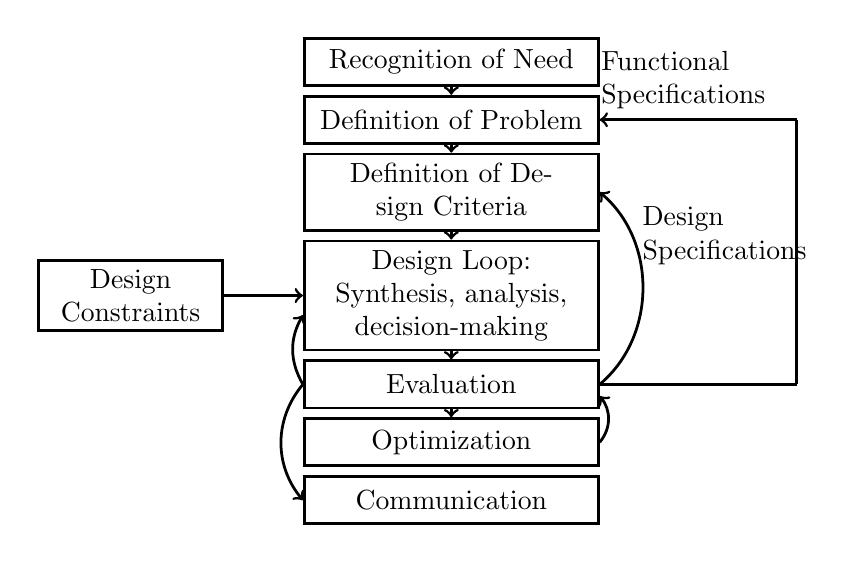
\begin{tikzpicture}[scale=0.5]
 \matrix (m) [matrix of nodes, column sep=1cm, row sep=0.1cm,
              nodes={draw, line width=1pt, anchor=center,
                     text centered, minimum width=1cm, minimum height=6mm},
              txt/.style={text width=3.5cm,anchor=center}
             ]
 { 
  & |[txt]| {Recognition of Need}  \\
  & |[txt]| {Definition of Problem}  \\
  & |[txt]| {Definition of Design Criteria}  \\
 |[txt, text width=6em]| {\begin{minipage}{6em}\begin{center}Design\\Constraints\end{center}\end{minipage}} & |[txt]| {Design Loop: \\Synthesis, analysis, decision-making}  \\
  & |[txt]| {Evaluation}  \\
  & |[txt]| {Optimization}  \\
  & |[txt]| {Communication}  \\
 };

 { [start chain, ->, every on chain/.style={join}, 
    every join/.style={line width=1pt}]
   \chainin (m-1-2);
   \chainin (m-2-2);
   \chainin (m-3-2);
   \chainin (m-4-2);
   { [start branch=constraints, <-]
     \chainin (m-4-1);
   }
   \chainin (m-5-2);
   \chainin (m-6-2);
 };
 \path[line width=1pt] (m-6-2.east) edge[->, bend right=40] ($ (m-5-2.east) + (0, -0.3) $);
 \path[line width=1pt] (m-5-2.west) edge[->, bend right=40] (m-7-2.west);
 \path[line width=1pt] (m-5-2.east) edge[->, bend right=50] node[near end,right] (ds) { \begin{minipage}{6em} Design \\ Specifications\end{minipage}}  (m-3-2.east);
 \path[line width=1pt] (m-5-2.west) edge [->, bend left] ($ (m-4-2.west) + (0, -0.5) $);
% \path[line width=1pt] (m-6-2.east) edge[->, bend right=80] node[near end,right] (ds) { \begin{minipage}{6em} Functional \\ Specifications\end{minipage}}  (m-2-2.east);
 \path[line width=1pt] (m-5-2.east) edge ($(m-5-2.east) + (5,0)$)
               ($(m-5-2.east) +(5,0)$) edge ($(m-2-2.east) +(5,0)$)
               ($(m-2-2.east) +(5,0)$) edge[->] node[above] (fs) {\begin{minipage}{7em} Functional \\ Specifications \end{minipage} }
                  (m-2-2.east);

\end{tikzpicture}
\end{center}

\end{frame}

\begin{frame}
\frametitle{Software is Different}

 
\begin{changemargin}{1cm}
Previous slide: a model for classical engineering disciplines---ends with
the transfer of blueprints to manufacturing and construction
firms. \\[1em]
\Large
Software is different.
\end{changemargin}

\end{frame}

\begin{frame}
\frametitle{Customer Requirements}

\begin{changemargin}{1cm}
In this phase:
\begin{itemize}
\item trying to figure out what the
customer is looking for.
\item note: customers might not know what they want;
\item can always give platitudes, e.g. convenient, easy-to-use, lightweight, simple.
\end{itemize}
~\\
By digging deeper, you can find a design problem among what they're
saying.\\[1em]

Avoid getting pigeonholed by ``helpful'' customers giving you advice on how
to solve the problem (but consider input).
\end{changemargin}

\end{frame}


\begin{frame}
\frametitle{Customer Requirements}

\begin{changemargin}{1cm}

Video:  https://www.youtube.com/watch?v=BKorP55Aqvg

\end{changemargin}

\end{frame}

\begin{frame}
\frametitle{Design Criteria}

\begin{changemargin}{1cm}
\begin{itemize}
\item Given a problem, you need to know
\emph{specifically} what constitutes a solution. 

\item Solution should, to the extent possible, meet the design criteria.

\item A project that fails to meet one criterion isn't necessarily a failure.
\end{itemize}
~\\

\alert{Examples of design criteria?}
\end{changemargin}

\end{frame}

\begin{frame}
\frametitle{Design Constraints}

\begin{changemargin}{1cm}
Constraints are what make things interesting
(as long as they're satisfiable). 
\begin{itemize}
\item Your task: find a constraint-satisfying
solution.
\end{itemize}
~\\

Design constraints may:
\begin{itemize}
\item apply to the design process (that is, the
designer or the final design) or the manufacturing process; 
\item be imposed by management, the environment, or physical laws involved
in the design.
\end{itemize}

\alert{What are some examples of design constraints?}\\[1em]

We usually consider design constraints non-negotiable; solutions must
satisfy all design constraints.
\end{changemargin}

\end{frame}

\begin{frame}
\frametitle{Heuristics and guidelines}

\begin{changemargin}{1cm}
Four related terms:
\begin{itemize}
\item \emph{design heuristic}: general (and not necessarily
actionable) rule-of-thumb based on experience.  \\[1em]

Heuristics lead to
quick design solutions that often work well but may fail in some
situations. \\[1em]

No substitute for understanding.\\[1em]

\item \emph{design guideline}: general rule based on experience and
specific knowledge of the design problem that may be applied to a design
solution. \\[1em]

More specific than heuristics.
\end{itemize}
\end{changemargin}

\end{frame}

\begin{frame}
\frametitle{Standards and Specifications}

\begin{changemargin}{1cm}
\begin{itemize}
\item \emph{standard}: provides more direction about the acceptable
solution space by stating technical requirements that must be satisfied
by candidate designs. \\[1em]

Do not provide a complete solution, but 
do dictate a set of requirements.\\[1em]

\item \emph{specification}: in this class, refers to a description of a solution
which provides all of the details. \\[1em]

Using a specification, an engineer
should be able to reproduce a design exactly.

\end{itemize}
\end{changemargin}

\end{frame}

\begin{frame}

\frametitle{Synthesis, Analysis and Decision-Making.}

\begin{changemargin}{1cm}
You've got constraints and requirements. Time to come up with a solution.
You will use the \emph{design loop}.

\begin{itemize}
\item \structure{Synthesis}: gather information, combine (synthesize) it, and come up
with ideas or methods to solve a problem.
\item \structure{Analysis}: estimate the expected result from each idea or method.
\item \structure{Decision-making}: compare the expected results and their uncertainties; pick the best alternative.
\end{itemize}
\end{changemargin}

\end{frame}

\begin{frame}
\frametitle{Iteration}

\begin{changemargin}{1cm}
\structure{Expect to iterate:}\\[1em]
\begin{itemize}
\item Even after you
get a ``best'' alternative, maybe your criteria were 
wrong, or you didn't satisfy all of the design constraints or meet
the desired design criteria.\\[1em]

\item When iterating, bring back less-favoured alternatives,
and reconsider and revise all of the alternatives. You'll get a better set
of alternatives.\\[1em]

\end{itemize}

Once you have a sufficiently-good best design, exit the
design loop. This design should satisfy all constraints and achieve the
desired criteria. \\[1em]

Choose the winning design, optimize, and implement.
\end{changemargin}

\end{frame}

\begin{frame}
\frametitle{Innovation versus evoluation}

\begin{changemargin}{1cm}
Solutions tend to have some
innovation and some evolution. It's a continuum.
\begin{itemize}
\item Evolutionary design solutions \emph{build on top of} existing solutions,
improving them in some way.
\item Innovative design solutions invent \emph{something new}, a completely
original idea or a novel way of solving the design problem.
\end{itemize}

Modern eng. design solutions combine innovation \& evolution.

(You don't want to innovate on all fronts simultaneously). 
\end{changemargin}

\end{frame}

\begin{frame}
\frametitle{Example: Brooklyn Bagel Slider}

\begin{changemargin}{1cm}
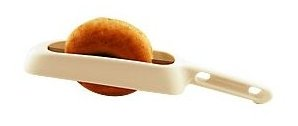
\includegraphics[width=.8\textwidth]{images/bbs.jpg}\\[1em]

Goal: Avoid Bagel-Related Injuries.\\[1em]

\alert{What is innovative about this design? What is evolutionary?}
\end{changemargin}
\end{frame}

\begin{frame}
\frametitle{Creativity}

\begin{changemargin}{1cm}
Popular misconception: engineering is not creative.

\begin{itemize}
\item Good engineering uses creativity
when necessary.
\end{itemize}

Know when to innovate and when to build on others' designs.\\[1em]

Avoid the high-risk, low-reward category: make sure there is a payoff,
and analyze your proposed solution carefully to ensure that it meets
all requirements and constraints.
\end{changemargin}

\end{frame}

\begin{frame}

\frametitle{Risks of creativity}

\large
\begin{changemargin}{1cm}
\begin{itemize}
\item adds to time required to complete a design; 
\item adds to cost for prototyping the design;
\item might not lead to a solution at all; and
\item might lead to an unsatisfactory solution.
\end{itemize}
\end{changemargin}

\end{frame}


\begin{frame}
\frametitle{The Creative Process: Synthesis/Analysis}

\begin{changemargin}{.5cm}
5 steps in a typical creative process:
\begin{enumerate}
\item Gather information.
\item Make a concentrated effort to understand the problem.
\item Take a break (sleep, do something else, take a shower, etc.)
\item Discover the solution to the problem (often subconscious).
\item Write down the solution and refine it.
\end{enumerate}
\end{changemargin}

\end{frame}

\begin{frame}
\frametitle{Tips for Creativity}

\begin{changemargin}{1cm}
How do you get something good?

\begin{itemize}
\item generate lots of alternatives.
\end{itemize}

(a.k.a. getting lots of practice developing 
skills\footnote{\tiny \url{http://www.lifeclever.com/what-50-pounds-of-clay-can-teach-you-about-design/}}\footnote{\tiny \url{http://www.lifeclever.com/talent-isnt-everything-7-habits-of-highly-effective-junior-designers/}})

~\\[1em]
Might not work as well:

\begin{itemize}
\item trying to come up with the one ideal solution.
\end{itemize}
\end{changemargin}

\end{frame}

\begin{frame}
\frametitle{Creativity: Brainstorming}

\begin{changemargin}{1cm}
\begin{itemize}
\item Synthesis: come up with new ideas synthesizing the information;
  don't discount any ideas, just write them down. [The usual part of
    brainstorming.]\\[1em]
\item Analysis: look at all of the ideas (to some extent) and analyze them. Determine the most promising solutions. [Also important!]
\end{itemize}
~\\

Because unusual ideas show up, and aren't immediately discounted, 
they can help you come up with a variety of creative solutions, some of 
which might be practical.
\end{changemargin}
\end{frame}

\begin{frame}
\frametitle{Creativity: Brainwriting}

\begin{changemargin}{1cm}
This is like brainstorming.

\begin{itemize}
\item Write down tentative solutions on \emph{solution sheets}.
\item Each team member picks a solution sheet to refine.
\item Exchange solution sheets until members run out of ideas.
\end{itemize}
Because you're writing things down, you can avoid dropping things on the floor.
\end{changemargin}

\end{frame}

\begin{frame}
\frametitle{Creativity: Pitfalls to Avoid I}

\begin{changemargin}{1cm}
Roger von 
Oech\footnote{\url{http://www.creativethink.com}} produces a lot of
output about creativity. 

Here are some misbeliefs, according to him:
\begin{itemize}
\item There is only one right answer.
\item The creative process must be logical.
\item They must ``follow the rules'' even if the rules are unwritten.
\item They must be practical and therefore inhibit their fantasies.
\item They must avoid ambiguity and therefore stifle their imagination.
\end{itemize}
\end{changemargin}

\end{frame}

\begin{frame}
\frametitle{Creativity: Pitfalls to Avoid II}

\begin{changemargin}{1em}
More misbeliefs:
\begin{itemize}
\item They avoid new ideas for fear of making mistakes.
\item Play is frivolous, and new ideas are hard work.
\item They narrow their focus and miss ideas in nearby areas.
\item They are not creative.
\item They are afraid to look foolish by suggesting an unworkable idea.
\end{itemize}
\end{changemargin}

\end{frame}

\section{Evaluation}

\begin{frame}
\frametitle{Evaluating Designs}

\begin{changemargin}{2em}
You have one or more candidate designs (design alternatives) and want
to see how good it is/they are.\\[1em]

A \emph{design review} is an independent evaluation of a design alternative:
\begin{itemize}
\item act as a ``sanity check'' on the design; and 
\item are often conducted by evaluation teams consisting of clients and/or
managers.
\end{itemize}
If all alternatives are bad (failed design reviews), the client might
terminate the project.
\end{changemargin}

\end{frame}

\begin{frame}
\frametitle{Questions for Evaluating Designs and Teams}
\begin{changemargin}{2em}
\begin{itemize}
\item Does the design team have a thorough understanding of the purpose and goals of the design?
\item Have all of the relevant requirements, criteria, and constraints been identified?
\item Is the overall design plausible for meeting the design objectives?
\item Does the overall design appear to meet the criteria specified?
\item Is the (anticipated) performance of the design adequate?
\item Are there any flaws in the analysis of the design?
\end{itemize}
\end{changemargin}

\end{frame}

\begin{frame}
\frametitle{Design Alternatives}

\begin{changemargin}{2em}
Consider presenting more than one alternative
at a design
review\footnote{\url{http://www.microsoft.com/design/article.aspx?type=stories&key=design}}. 

\begin{itemize}
\item Life is often unclear.
\item Alternatives: customer has a choice,
\item rather than saying ``I don't like that!''
\end{itemize}

Trying to push bad designs forward can help you understand why those
designs are bad.
\end{changemargin}

\end{frame}

\section{Communication.} 

\begin{frame}
\frametitle{On Communication}

\begin{changemargin}{2em}
Communication is the final phase in traditional engineering
disciplines.\\[1em]

(Not so in software!)

\begin{itemize}
\item You
haven't done anything if you don't (successfully) tell anyone about
it. 
\item Communication is also important en-route.
\end{itemize}
\end{changemargin}

\end{frame}

\begin{frame}

\frametitle{Who To Communicate With?}

\begin{changemargin}{2em}
\begin{itemize}
\item Between Stakeholders: Designers/implementers, managers, and clients.\\[1em]

Default assumption: things are going well. \\ May lead to unhappiness.\\[1em]

\item Intra-Team Communication. 
\begin{itemize}
\item Small team:
helps with continuity; allows you continue the project even if an
engineer leaves the company. 

\item Large team: mandatory for making sure that all parts
integrate and for tracking the schedule.
\end{itemize}
\end{itemize}
\end{changemargin}

\end{frame}

\section{Design Team Organization}

\begin{frame}

\begin{changemargin}{2em}
\frametitle{Tips on Organizing Design Teams}

\begin{itemize}
\item Keep teams small, e.g. ``two-bit'' teams.

Larger teams have too much coordination overhead.
\item Think about dividing responsibility. 
\item No useless work.
\item Open communication; track progress. (Don't pester!)
\item Encourage creativity when necessary, but make sure team members
  aren't going overboard.
\end{itemize}
\end{changemargin}
\end{frame}

\begin{frame}
\frametitle{Two Pizzas}
\begin{changemargin}{1cm}
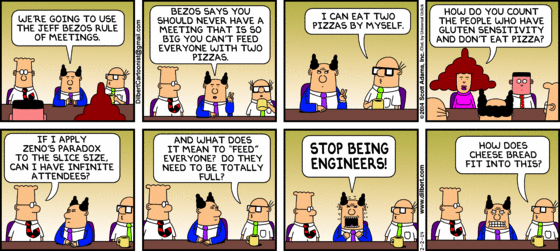
\includegraphics[width=.8\textwidth]{images/twopizzas.png}
\end{changemargin}
\end{frame}



\begin{frame}

\frametitle{Potential Dysfunctions}

\begin{changemargin}{1cm}
Per Steve McConnell, \emph{Rapid Development}, 
pp. 156--168, Microsoft Press, 1996.
\begin{itemize}
\item Lack of common vision
\item Lack of identity
\item Lack of recognition
\item Productivity roadblocks
\item Ineffective communication
\item Lack of trust
\item Problem personnel
\end{itemize}
\end{changemargin}

\end{frame}

\begin{frame}

\frametitle{Typical Set of Design Groups}

\begin{changemargin}{2em}

\begin{itemize}
\item \alert{Development Group}: tests the feasibility of new technologies and ideas.
\item \alert{Design Group}: refines a design to ensure manufacturability, reliability, safety, and efficient operation.
\item \alert{Manufacturing Group}: refines a design based on the results of the manufacturing process and the performance of test~batches.
\item \alert{Quality Control Group}: monitors the quality of products in wide use.
\item \alert{Customer Service Group}: tracks the performance of products and ongoing maintenance performed for customers.
\end{itemize}
\end{changemargin}

\end{frame}

\begin{frame}

\frametitle{Comments on Design Groups}
\begin{changemargin}{1cm}
Design groups work concurrently and synchronize with each other.\\[1em]

Groups have different goals and deadlines---consensus and
cooperation may be difficult to achieve. \\[1em]

(Organizational inertia generally makes cooperation difficult, even
without different goals and deadlines.)\\[1em]

Project management: get everyone working together.\\[1em]

Time management is particularly key.
\end{changemargin}
\end{frame}

\end{document}
